
\chapter{绪论}
\label{chap:introduction}
\section{研究背景与意义}
	互联网自二十世纪九十年代从诞生、发展,到现在已经演化为人类社会的必需品。随着互联网的发展,用户的信息检索模式也发生了翻天覆地的变化,早期用户可以毫不费力的直接记住寥寥无几的网站、网址,轻松实现上网需求;随着网站呈指数的发展,网址数量大大超出人脑记录的容量,于是Yahoo!公司首次提出并实现了分类目录系统的概念,其本质还是通过人工将网站分门别类,因此其创新还是属于量变,没有达到质变。随着网站进入到爆发式增长,人工进行分类目录法变得越来越不现实了,于是产生Google为代表的搜索引擎,搜索引擎实现了互联网的质变,通过程序自动化的实现了检索网站、爬取内容、存储数据,实现了亿万级的数据积累,只有基于如此庞大的信息,才能为哪怕是最普通的用户提供及时、准确、快速信息获取服务,人类社会一定程度上填平了所谓的“信息鸿沟”。但是,后互联网时代又是个性化时代\citep{Personalization1,Personalization2,Personalization3,Personalization4,Personalization5,Personalization6,Personalization7,Personalization8,Personalization9},需要一种系统精确刻画每个用户的兴趣爱好并能不动声色的在主页上表现出来,我们把这种提供个性化服务的系统系统统称为推荐系统。推荐系统是一种比搜索引擎更人性化、个性化的系统服务,不需要用户主动提供关键词,因此它能满足用户的更多的潜在需求,尤其当用户自己都无法精准描述自身需求的时候\citep{recmd-system}。第一代推荐系统以亚马逊为代表,作为一个电子商品平台,一方面有数以万计的商品需要被用户了解、熟悉和购买,另一方面有数以亿计的用户无法找到称心如意的商品。推荐系统通过构建用户和商品之间的桥梁,每年为亚马逊贡献近三十个百分点的创收!由此可见推荐系统能帮助用户快速发现有用的商品信息,具体来讲,首先推荐系统通过分析用户的历史行为每个用户进行独一无二的画像建模\citep{demo-data},目的有俩个:1,熟悉每个用户和他们的潜在需求;2,把拥有相同品味的用户归为一类群体,这样一来所有人的需求总和就可能是其中一个人的潜在需求,方便企业卖出更多的商品。随着用户终端设备的普及,出现了诸如淘宝、美团、滴滴、今日头条等互联网平台,几乎包办了人们衣食住行的方方面面,人们因为可选择性太多而出现了“选择性困难”的症状,这其实就是信息过载时代的具体表现形式。也就是说,在这个数据爆炸时代,无论是作为信息消费者的普通用户,还是作为信息生产者的提供商,都面临着日益严峻的挑战,现代人每天面临着从各种不必要的数据中找到有用的商品,其实是在浪费生命。每一个有追求、有理想的现代人,真的需要好好的设计人生,以一种精要的方式摒弃不必要之事,而这也是林语堂先生所说的生之智慧。笔者曾有过这样的一种购物体经历:笔者在淘宝商城购买一台笔记本电脑,花费了一上午的时间才浏览、比较完所有的 thinkpad 品牌商家店面,如\autoref{fig:hl_taobao}。
	\begin{figure}
		\centering
		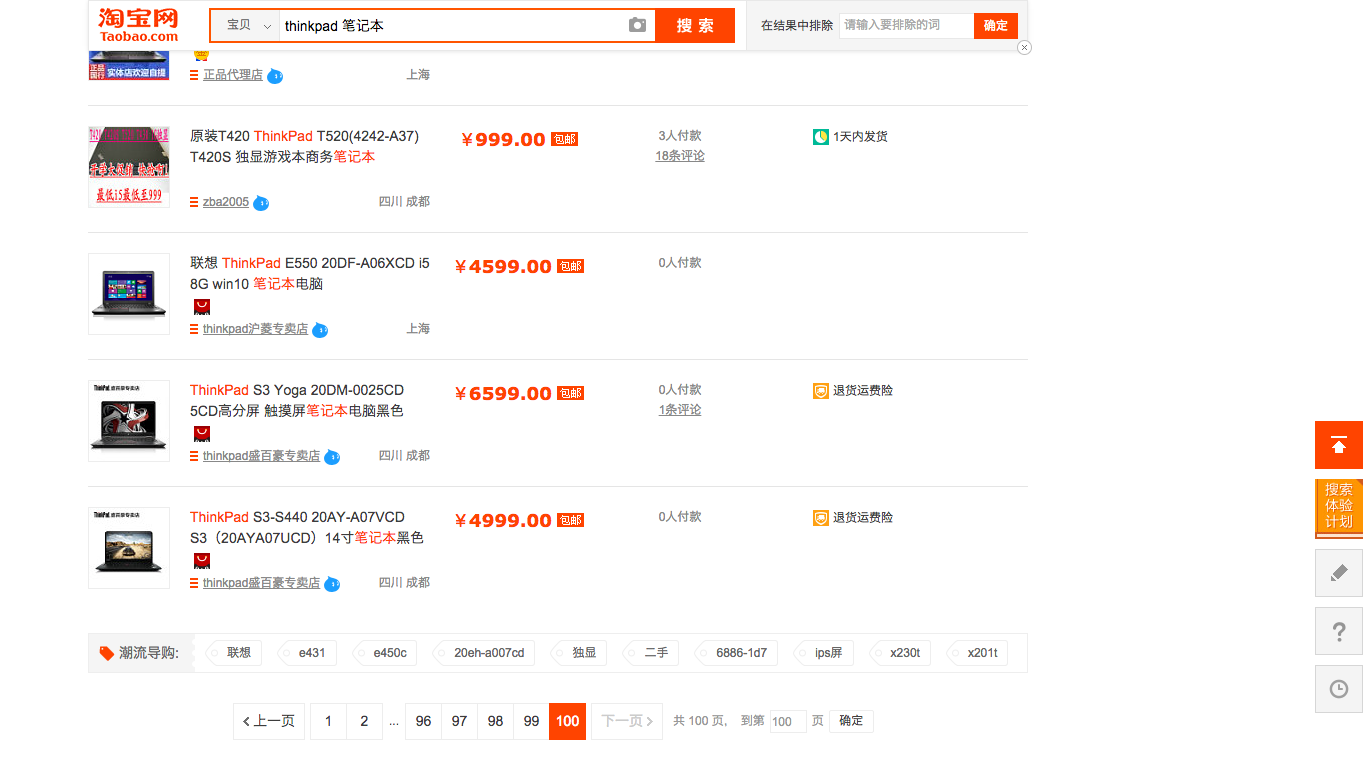
\includegraphics[width=0.9\textwidth]{hl_taobao}
		\figcaption{淘宝购物搜索图}
		\label{fig:hl_taobao}
	\end{figure}
	其实,作为互联网电子商家的翘楚---淘宝,一直在思考如何让自己平台下的优秀商品不埋没在大数据洪流中,因此,淘宝技术团队一直把个性化推荐系统视为解决用户-商品合理匹配的终极杀手锏。对于一个电商平台,原则上商品肯定是多多益善,但对于一个个性化推荐系统,则遵守更少,但更好的原则,推荐系统代表了一种自律的、精要的生活方式,据笔者所知,已经有很多互联网企业已经或者正在开发符合其企业文化的推荐系统,如笔者曾供职过的小米、今日头条和滴滴出行,其中小米的广告部门很早就利用推荐算法实现旗下各个业务线的智能广告投放,而今日头条利用推荐系统每日为用户定时推荐文章,滴滴出行则利用推荐系统为每个乘客和网约车做定向最优推荐。对于传统的推荐系统,首先,需要积累足够多的商品信息,因为只有尽可能的在基于所有的商品大局观上,才有可能得出比较正确的商品推荐候选集合;其次,需要尽可能积累用户的行为样本数据,因为这些样本将会是推荐统计假设检验的唯一数据标准,统计学之所以常让人意外,就是因为人们只能得到部分样本,而部分样本只是包含了事情的部分信息,于是就有扭曲事情本质的趋势,因此,精度是推荐系统最重要的指标之一,后文会详细介绍如果通过用户画像和用户兴趣\citep{user-interests-explore,user-interests-explore1,user-interests-explore2,user-interests-explore3,user-interests-explore4}提升推荐系统的精度;最后就是甄别,哪些商品对哪些用户有着非同寻常的吸引力,其实对于一个用户来讲,平台上存在的绝大多数商品,包括数据、资源和他人观点,都没有什么价值,只有少数商品效果非凡,影响巨大,推荐系统的核心就是算法\citep{date-mining},通过算法甄别无意义的多数,只留下有意义的少数。总之,通过算法分析用户兴趣,分析商品特性,对用户跟所有商品的关联度打分、排序、取topN,然后给出推荐结果。

	但是,传统的推荐系统也有一些问题,典型的有数据稀疏问题、新用户问题、马太效应、实时推荐问题和用户兴趣变动问题。数据稀疏问题的本质就是商品信息数据过于膨胀,即使是骨灰级用户也没办法穷尽百分之一的商品,因此大多数的用户-商品相关值都是零,这不利于推荐系统做出正确的推荐结果;新用户问题又叫冷启动问题,指一个用户刚刚注册登录,推荐系统没有与此人相关的信息,于是就没有方法做出推荐;马太效应是指越热门的商品越有被推荐的趋势,这种情况其实不是一件好事,因为:1,商品营收不平衡会增加平台的风险性,如果平台大多数营收的贡献来自于极少类明星商品,一旦这类商品发生问题,平台也会有问题;2,根据2/8原则,冷门商品虽然营收少,但它们的基数大,潜力无限;实时推荐问题是指用户从浏览到购买这段时间一般很短,而推荐系统需要打时间差,在用户点击之后、购买之前的这段时间做出推荐,但这是很难实现的,一个客观原因是对所有商品打分、排序、取 topN,最后找到用户感兴趣的商品,在工程上是需要一些时间的;用户兴趣变动问题是指用户兴趣是一个动态的过程,有可能随着季节周期性变动,有可能随着年龄发散性变化,推荐系统需要及时收集数据,保持对用户兴趣的最优拟合。

	基于这些问题的存在,笔者基于推荐系统实现了用户画像模块和用户兴趣探索模块,用以解决传统推荐系统所面临的种种问题,并帮助推荐系统做出更好的推荐结果。用户画像模块其实就是回归了问题的本质:以人为本,用数据说话。通过分析、收集所有与用户有关的数据,为每个用户建立、维护一个独一无二的用户画像,用户画像的最大优点在于它能主动收集用户的基本人口数据、长期兴趣和短期兴趣,而且用户画像中的信息是动态更新的,也就是说随着时间的推移,用户的兴趣在逐渐改变,用户画像里的兴趣标签也会随之改变,最大程度上保证了用户兴趣的连续性和变化性;用户兴趣探索模块包括三个原则:1,用户和潜在感兴趣商品的关联度很低,这保证了探索的商品都是用户从前没有看见过的;2,用户满意度很高,即通过量化用户行为,包括点击次数、滑屏次数、滑屏频率、滑屏时长、点赞、分享等行为,得出用户的满意度;3,潜在商品的标签是小众的、冷门的标签,因为热门商品是没必要也不需要做探索的。

\section{推荐系统的简介}
推荐系统的研究其实是个交叉学科,因为其跟很多早期的基础领域的研究相关,比如认知科学\citep{cognitive-science},信息检索\citep{info-retrieval}和预测理论\citep{Forecast-principle}。随着数据时代的到来,研究人员开始研究如何利用用户对商品的行为数据来预测用户的兴趣,同时为用户提供推荐服务\citep{cf-sn}。近些年来,推荐系统越来越开始成为一个专门的研究课题,到2005年左右为止推荐系统的研究还是集中在基于user、item的协同过滤算法\citep{Wikipedia},在工业界目前应用最具有影响力的算法应该就是亚马逊的协同过滤算法\citep{Amazon-cf}。推荐系统推荐有俩个原则:1,给用户的商品不能与用户购买过的商品重复;2,不能与用户刚浏览过的商品太相关。推荐系统的函数形式化定义:设C是所有用户的集合,S是所有可以推荐给用户的主题的集合。实际上,C和S集合的规模通常很大,如亿级别的顾客以及百万级别的商品。设函数u()可以计算主题s对用户c的推荐度R,即$u=C\times S \rightarrow R$,R是一定范围内的全序的非负实数,推荐要研究的问题就是找到推荐度R最大的那些主题S*,如\autoref{equ:fromal}。
\begin{equation}
\forall c \in C,S^{*}=arg  max_{s \in S} u(c,s)
\label{equ:fromal}
\end{equation}

	\subsection{推荐系统的产生与发展}
	随着计算机存储技术以摩尔定律指数增长,信息的传播也开始爆发式的迅猛发展起来,我们这个时代的人类社会进入了一个崭新的大数据信息时代:互联网和物联网几乎无处不在,影响人类的衣食住行等方方面面,因此颠覆性的更改了人们的生活方式,在典型的互联网共享经济平台,一个用户既代表了消费者,也代表了生产者,就如笔者在滴滴出行的角色,平时上下班打车,属于运力消费者,周末开车做网约车司机,则变身为运力生产者。但是不好的一方面也开始浮现,曾几何时笔者发现自己社交账号开始多起来,数量之多以至于没办法记住每个账号的密码。这就是Web 2.0时代的一个副作用---让人们疲于奔命的把生活浪费在刷各种动态、信息,忙于各种无脑点赞、分享,而没有时间思考。社交化网络媒体如微信、微博的异军突起,导致互联网中的信息数据中充满了广告和噪声,而普通用户一般缺少过滤、屏蔽噪声的主观意愿和技术能力,不仅使其信息检索的时间成本巨大,也会让其在茫茫多的数据海洋里迷失自我,这就是信息过载问题的根源所在\citep{info-overload, info-overload:1}。作为非常重要的技术手段,推荐系统和搜索引擎为用户解决信息过载提供了不可或缺的保障。倆者的不同之处在于:搜索引擎是分散的、被动的,用户需要先输入关键词,搜索引擎根据关键字在服务器后台进行信息检索,利用算法获得最优的匹配信息并展示给用户。但我们更多时候遇到的问题是,并不能精确描述自己的需求,而这就是推荐系统的强项,因为推荐系统是主动收集用户平日中一点一滴的数据,以至于用户不需要提供明确的需求,推荐系统只是通过分析用户的历史行为数据就可以“猜出”用户的意图,因此,如果我们把推荐系统和搜索引擎看作为两个互补的技术手段,那么效果一定很棒。

	推荐系统最开始的概念,应该是在1995年由美国人工智能协会\citep{recmd-history}上的Robert Armstrong教授首先提出,不仅如此,Armstrong教授还不遗余力的推广了一个推荐系统的原型系统。受其启发,推荐系统的研究工作开始起步并发展壮大。第一个商用推荐系统应该属于Yahoo网站的个性化入口MyYahoo。到了21新世纪,随着电子商务的风起云涌,推荐系统的研究与应用开始水涨船高,包括eBay、taobao、Amazon、youtube\citep{recmd-youtube}等各大电子商务网站都有了自己的推荐系统,其中,Amazon公司称其网站中百分之三十的营业额的流量入口来自于推荐系统。2006年美国的Netflix\citep{recmd-netflix}在网上公开了一个推荐算法竞赛,设立了丰厚的奖金,选手通过利用Netflix公开了的真实网站中的一部分数据,包含用户对电影的评分,利用数据挖掘算法预测哪些用户会购买哪些电影。2014年阿里举办了阿里大数据竞赛,笔者和小伙伴有幸参加并顺利进入决赛,阿里公开了其部分用户三个月的浏览、收藏、购买商品数据,选手可以利用阿里天池计算资源做出预测,阿里大数据竞赛有效地推动了学术界和产业界对推荐算法的兴趣,很多有效的算法在此阶段被提了出来。

	随着互联网企业深入人心的发展、壮大,推荐系统在电子商务中的优势地位也越来越明显。国内比较典型的电子商务平台网站有淘宝网、网易云音乐、爱奇艺PPS等。在这些电子商务平台中,网站提供的商品数量不计其数,网站中的用户规模也是亿级别的。据双十一官方统计,天猫商城中的商品数量已经超过了5000万。试想下,在如此庞大商品数量的电商网站中,如果用户仅仅依靠搜索引擎输入关键字查询,只是过滤了百分之九十九的商品,对剩下百分之一的商品还是没辙。淘宝网在这一块做的很好,其手机app主页的推荐系统能够根据用户浏览行为\citep{user-interest}及时的为用户推荐商品,笔者发现淘宝的推荐结果已经成为大部分用户的主要购买入口,总的来说,目前比较成功的电子商务网站中,都在利用推荐系统这只会下金鸡蛋的母鸡,在用户购物的同时为用户推荐一些商品,从而提高商品的销售额。另一方面,随着以IOS、Android系统为代表的物联网引领了移动互联网的发展潮流。在用户在接入移动互联网过程中,其经纬度信息可以被非常准确地被获取,因此出现了大量的基于用户位置信息推荐系统。国外比较著名的有Uber和Coupons。国内著名的有滴滴出行和美团网。美团网这种基于互联网的外卖平台,会利用位置服务为用户可推荐当前位置的餐馆、酒店、影院、旅游景点。线上交易,线下消费,之后为自己在现实世界中的体验打分,分享自己的经验与感受,形成线上下单-线下消费-线上评价的生态闭环。只是当笔者使用美团基于位置的美食服务时,同样也会遭遇信息过载问题,矛盾在于商家太多了,而笔者只能一次去一家餐厅就餐,这时美团平台的推荐系统会根据笔者的历史消费信息,加上笔者的偏好、口味、消费能力等,为笔者推荐当前位置下最可能感兴趣的餐厅。

	随着网络社交的深入人心,用户不再满足于单纯的获取信息,而是与网络上的其他用户进行关注、聊天和互动。国外著名的社交网络就有Twitter、Facebook等,国内的社交网络有微信、微博等。在社交网站中用户不再是一个静止端点,而是与他人有错综复杂关系的社交网络。对于微信来说,最重要的资源应该就是用户之间的关联。这其中的关系可能是多层次的、多维度的、按时间序列走的,关联的因素可能是是亲人、好友、同学、同事,也可能只是网络中的萍水之交,如都是QQ黄金会员。因此,用户之间的关联应该有一个权重,表明了用户之间的紧密度、信任度,一个用户的好友可能是另一个好友的亲戚,因此推荐系统有助于帮助用户挖掘潜在的熟人。

	同样自推荐系统诞生后,学术界对其的关注度一直不小。从1999年开始,在美国每年由计算机学会负责召开电子商务研讨会,会中已经发表了数以千计的推荐系统论文。在2001年,ACM信息检索专业组考虑把推荐系统独立拆分,作为会议诸多独立研究主题之一。2001年同年,在人工智能联合大会上,推荐系统也单独列为一个主题。2011年的KDD CUP 竞赛中,两个竞赛题目分别为音乐评分预测和识别音乐是否被用户评分(\href{http://www.kdd.org/kdd2011/kddcup.shtml}{www.kddcup2011.org})。2012年的KDD CUP 竞赛中,两个竞赛题目分别为腾讯微博中的好友推荐和计算广告中的点击率预测。(\href{www.kddcup2012.org}{www.kddcup2012.org})

	\subsection{推荐系统的应用}
	作为IT数据挖掘算法工程师,笔者经常听到同事开玩笑的说:推荐系统就像万金油,抹哪哪灵。对于诸如linkedin的社交网络,推荐系统改变用户扩展人脉的模式和方法,而这是基于一种假设:你的朋友的朋友有可能就是你熟悉的人。对于诸如淘宝的电商平台,搜索提供的静态体验,并不足以让用户产生购买欲望,推荐系统加强了交互,包括用户和商品、用户和用户,一个人的消费可能带动一群人模仿,成就了一种极致的营销模式。对于诸如滴滴出行的网约车平台,给定某一时刻、起始经纬度、终点经纬度、车型,根据推荐算法一定会有一个最优派单,使得司机和乘客所得的好处,远远大于平台的抽成费用,形成了我们所说的三方共赢,只有“倒霉”的传统出租车利益受损的局面。总体说来,一个成功的个性化推荐系统的应用主要表现在以下几个方面:
	\begin{enumerate}[(1)]
	\item 将潜在用户转变为购买者:用户在浏览的同时并不意味着一定是要消费,也许只是看看,遇到合适就买,没有就算。个性化推荐系统的职责之一是能够洞察用户的潜意识,帮助用户找到其感兴趣的商品,从而促成购买过程。
	\item 提高平台的连带销售能力:有时候个性化推荐系统需要一点联想能力,如用户购买了手机,那么推荐手机壳就是一种明智的联想,会让用户产生“你懂我”的感觉。
	\item 提高客户对平台忠诚度:个性化推荐系统就是那个时时刻刻为用户着想的机器人,每一次推荐只是那么一点点,不是很多,但都很好,这种依赖就是俞军先生所说的体验壁垒,对于用户来讲,从滴滴出行换到Uber,功能还是原来的功能,只是用户习惯的打车方式都变了,以至于无法接受Uber。
	\end{enumerate}

\section{用户画像的简介}
	用户,指企业的潜在消费者,是构成现有用户的大部分群体的统称。画像,是对一个用户的可视化、客观的描述。用户画像就是能够客观、可视化地描述潜在消费者的模型。用户画像建模的关键工作就是为用户打上合适的标签,标签通常是人为规定,且具有高度精炼的特征标识,如消费能力、偏好、年龄、性别等,将所有用户标签综合起来,抽象出本质,如忠诚度、消费度、满意度等,基本就可以勾勒出该用户的商业消费轮廓。
	\subsection{用户画像的产生背景}
	当互联网步入信息时代后,用户行为数据的极大丰富性给企业及消费者的消费行为带来一系列问题与变革。最大的问题在于电子商务的用户数量相比传统商务,膨胀了成百上千个数量级,单纯依靠人工方式已对其无解,2015上半年,我国网民已达到6.68亿,预计年底能够顺利突破7亿,其中使用手机上网人群占整体88.9\%,而手机上网存在着独特性、唯一性和私密性的特点,每个人的手机都是一套独特的生态系统。最大的变革莫过于,消费者的一切行为信息都是可数字化,随着大数据工程技术的日益精湛,带宽、计算资源、存储资源也变得极大丰富起来。这使得企业有能力把专注点回归到问题的本质,即利用信息化管理方式为每位用户建立一个档案,根据用户的生活习惯、消费行为和社会属性等信息,抽象出的一个标签化的用户模型用以精准刻画用户,基于此进而充分挖掘用户潜在的商业价值,随着用户使用时间越长,模型就越能积累多的数据,也越能精确把握用户的消费习性,反过来越能促使用户的消费行为,形成一个良性循环,至此用户画像的概念也就深入企业和用户之心。

	大数据时代的用户行为数据就像是做饭的米,如果想让其变成香喷喷的白米饭,还面临很多问题:1、用户行为数据通常包含了很多的噪声,包括用户无目的地的浏览数据、用于营销目的的分享数据、用于作弊的刷单数据等等,这些数据并不能够代表用户的真实意图甚至有时代表的是相反的意愿;2、用户行为数据通常需要将其所包含的意义抽象化,才有利用价值,比如根据用户最近一个月的浏览、购买记录,通过分析、抽象、挖掘得出用户的活跃度、消费能力和忠诚度,这才能为算法所用;3、用户行为是是一个不断迭代的行为,如何均衡新旧行为数据的权重比,是一个很严肃的问题,比如一个用户上一个月购买不断,最近一个月却很少登录,那么我们应该怎么归因用户的这种行为?以及如何刻画这个时期的用户消费状态?如果用户处于将要流失的状态,又该如何做;4、不管到哪,我们总会遇到与自己志同道合的其他用户,我们其实还是比较关心这些人的选择,如果能拿来做为自己的参考也不是一件坏事,因此,如果存在一种机制,可以将有相同特征的用户抽象成一个代表,进行交叉推荐,则既方便用户消费又能促进企业营收。基于以上种种问题,我们确定选用了用户画像。
	\subsection{用户画像的应用}
	用户画像建模的过程,就是数据清洗、数据分析、数据挖掘,最后得出用户的抽象概念的过程,用户画像的本质就是了解企业的用户,然后完善产品运营提升用户体验,提升盈利,用户画像可以为包括推荐系统、运营推广、策略制定等提供数据支持。除此之外,用户画像可以帮助企业寻找潜在目标用户,在与用户的交互上了解其偏好,促成购买,实现精准运营和营销,用户画像改变了以往闭门造车式的商业交易模式,通过事先调研用户需求反馈,设计制造出更适合用户的产品。具体来讲,用户画像的应用包括:
	\begin{itemize}
	\item 完善及扩充用户信息:用户画像代表了用户的信息全貌,因此寻找足够多的数据是用户画像建模的前提条件。我国在各方面都是很大的长尾市场,互联网很大程度上弥补了信息的不对称,移动互联网又让把信息在精准送达到任意一个用户面前,尽管如此,根据2/8原则还是导致了大多数的用户和商品的数据是空缺着的。同时,在实际中用户的信息也可能提供得不尽完整,如对于没有填写性别信息的用户,用户画像可以通过用户兴趣探索模块,生成用户数据,可见,用户画像不仅消费数据,也可以生成数据。
	\item 打造健康的生态圈:在掌握用户信息的基础上,电子商务平台就可以对自身的状况进行分析,从相对宏观的角度刻画用户种群的分布,从基础上把握市场的生态环境,挖掘出商品的最大价值,帮助企业提高收入。例如笔者曾经发现,通过与当前热门电影保持同步,通过适时发布引导疯传引爆点、跟进推广周边手机主题,可以很好的带动用户的消费行为,用户的消费与此同时也刺激了第三方设计师紧跟时尚潮流,尽可能第一时间发布引领流行的作品。
	\item 支撑推荐系统的精准推荐:精准推荐的前提是对用户的清晰认知。在实际场景中,影响用户对商品的使用黏度的因素很多,在这种情况下,利用用户画像可以对用户的“贴身跟踪”就能及时发现薄弱环节,因此从用户打开应用网上商店到退出使用,其间的每一步情况都被快的记录在案:哪一天退出的,哪一步退出的,退出之后“跳转”到什么软件等等。据此,用户画像也实现了用户另外一个纬度的归类,分清哪部分是忠实用户,哪部分可能是潜在的忠实用户,哪些则是已经流失的;更进一步来看流失的原因:因为代金券没有了流失?主题包质量不好流失?这些都是下一步精准推荐的依据,无论是基于兴趣的推荐提升用户价值,精准的广告投放提升商业价值,还是针对特定用户群体的内容运营,用户画像都是其必不可少的基础支撑。
	\item 市场安全领域的应用:有时候商家会通过各种活动形式的补贴来获取用户、培养用户的消费习惯,但同时也催生一些通过刷排行榜、刷红包的用户,这些行为距离欺诈只有一步之遥,但他们的存在严重破环了市场的稳定,侵占了活动的资源。其中一个有效的解决方案就是利用用户画像沉淀方法设置促销活动门槛,即通过记录用户的注册时间、历史登陆次数、常用IP地址等,最大程度上隔离掉僵尸账号,保证市场的稳定发展。
	\end{itemize}

\section{工程背景}
	小米科技有限公司作为国内发展较快的互联网企业,活跃用户过亿,移动端用户比例高,有着大量的用户和丰富的用户行为,这些为推荐系统的应用和优化提供了不可或缺的条件,我们基于MIUI主题应用商店开发的手机主题推荐系统,作为用户和主题包之间的桥梁,体现出超强的变现能力。但现有的手机主题推荐系统也面临着一些问题。
	\begin{enumerate}[(1)]
	\item 新用户冷启动问题。当前使用的推荐算法,包括最近邻的协同过滤算法、PageRank排序算法、关联规则挖掘是根据给定用户对某些物品的行为数据,给每个用户推荐Top-N个其最喜欢的物品,当一个新用户进入一个站点时,我们对他的兴趣爱好还一无所知,这时如何做出推荐是一个很重要的问题。现有的机制是向用户推荐那写普遍反映比较好的物品,也就是说,推荐完全是基于物品的,这就会使热门的商品越来越热,冷门的商品越来越冷,代价就是加剧了热门商品的马太效应。

	\item 数据稀疏问题,通过观察我们发现只有约20\%的用户有过多于5款/日主题的浏览记录,意味着大多数用户的消费处于待挖掘状态。与此同时,我们发现只有约20\%的主题包有过多于10次/日的浏览次数,意味着大多数主题包的消费处于待挖掘状态,又是一个“蛋和鸡”的问题:要形成好的推荐,首先需要有大量的用户行为支持,这样才能得到足够多的推荐数据,这里问题的关键在于推荐系统如何首先能在数据稀疏的情况下给出优质的服务,打破闭环。

	\item 不断变化的用户喜好,这个问题主要分为俩类:1、用户一直喜欢某种类型的主题包,只是长时间没有机会接触,如一位男性用户喜欢美少女主题包款式,虽然不会主动查找,但如果不经意看到一款制作精美的美女主题包,可能还是会购买,这就是用户的长期兴趣。2、用户之前喜欢某种类型的主题包,之后转为喜欢另外一类主题包,如用户刚开始喜欢清纯系,后来转为温柔系,这时如果向用户推荐温柔系主题包更有可能被其接受,这就是用户的短期兴趣。

	\item 重复推荐的问题,手机主题包属于电子虚拟商品,它的特性是第一次下载需要购买,之后下载则免费,现有的推荐系统会重复推荐用户之前购买过的主题,导致占用有限的推荐位来显示无法变现的信息,并且会给用户一种不专业、不智能的体验。

	\item 其他问题,如推荐商品长尾性\citep{long-tail}有待加强、隐性喜好\citep{latent-cf}难以挖掘、偏激的用户和另类的产品、推荐系统的作弊行为、用户请求量大等。这些问题相对来讲影响范围小,本论文不做过多讨论。
	\end{enumerate}

	我们发现,如果在底层数据仓库层和推荐系统之间加一个用户画像模块,会有效提升推荐系统的各项性能。1、对于新用户冷启动问题、数据稀疏问题,关键是收集足够多的用户基本信息,在没有或者只有少量用户行为的情况下依靠用户画像对用户推荐比较合理的主题。2、对于不断变化的用户喜好,我们通过用户画像存储用户用户长期,通过用户兴趣探索获得用户短期兴趣,并针对手机主题市场的特点,利用线性衰减算法融合用户画像和用户兴趣探索,使得推荐结果能兼顾俩者。3、对于重复推荐的问题,我们在用户画像中维护一个白名单,用来存储用户曾购买过的所有主题信息,格式为(userId,itemId,buyTime)这样的三元组,避免向用户推荐已购买过的主题。除此之外,我们也通过探索用户小众兴趣提升推荐系统的长尾发掘能力,加强了对小众主题包的推荐力度。主要思路是分析用户所有的行为数据,针对占大多数的冷门主题(即包含小众标签的主题)会赋予一个倾斜因子,这样会使得冷门主题更有可能被探索出来。

	总之,我们采用构建用户画像的办法分析、处理、挖掘现有的用户信息,尽可能多的识别用户基础特征和兴趣偏好,达到精细化推荐的目的,包括后续定向广告投放、市场营销等功能需求也都是围绕建立更细致、准确的人群画像而展开。
\section{推荐系统开源项目介绍}
工欲善其事,必先利器,关于大数据,有很多令人兴奋的事情,但如何分析、利用好如此多的数据也带来了很多困惑。好在开源观念盛行的今天,有一些在大数据领域领先的免费开源技术可供利用。
\begin{itemize}
	\item Redis:Redis是一个remote类型的内存数据库,它不仅性能强劲,可扩展性好,而且还具有高效的复制特性,生来就是为解决实际问题而设计的数据模型。在实际工程中,笔者利用redis做俩件事情:1、存储计数指标,包括用户浏览、下载、购买等行为的次数,以天为单位,因为内存有限只存储最近一个月的数据;2、存储最近俩周的行为数据,按照timelines格式存储,天然支持时间排序。key有用户id,商品id,交易id,value格式为商品类型:商品价格:折扣,score为下单时间戳。
	\item Apache Hadoop:Hadoop是由大名鼎鼎的Apache基金会所开发、维护的一个分布式系统,是第一款开源的用于分布存储大型数据集的开源框架,助力各企业迅速从海量数据中挖掘出“金子”。在实际工程中,每日凌晨,把当日的MySQL DB中的数据复制一份到hdfs文件,partition为当天时间。
	\item Apache Hive:Hive是著名社交网络公司facebook开源的在Hadoop上的数据仓库基础构架。Hive的使用方式如传统的DB,类似SQL查询语言。同时,hive也帮助用户屏蔽具体的 MapReduce开发,因此十分适合大量数据的统计分析。实际工程中,笔者利用hive计算超过一个月的数据计算,其小时级别的计算时间限制了其只能适用于离线计算。
	\item Apache Spark:Spark是加州大学伯克利分校所开源的基于内存的通用并行计算框架,同时spark如hadoop一样容易扩展,因此适和完成数据挖掘需要大量计算迭代的任务。实际工程中,笔者利用spark自带的机器学习mllib库做推荐系统的模型训练。
	\item Apache Kafka:Kafka 是美国求职社交公司linkedin开发、开源的一种高吞吐量的分布式发布订阅消息系统,可以轻松处理现有所有大交易规模的用户行流数据,包括今日头条、滴滴出行级别的交易量都是利用kafka做导流。kafka的一个应用特点是实时性高、吞吐量巨大,任何要求实时处理的应用场景,Kafka都是一个可行的解决方案。实际工程中,笔者利用kafka流作为redis数据的上游数据源。整体数据流结构为:app->mysql db->mysql binlog->kafka->清洗、去重kafka->redis。从app到redis理论延迟为毫秒级别,其中的kafka是关键实现部件。
\end{itemize}

\section{论文结构}
	本文的其余正文内容由以下章节组成:
	\begin{itemize}
		\item 第二章首先介绍了推荐系统基本概念,然后详细介绍了用户画像和用户兴趣探索。
		\item 第三章主要讨论了如何利用用户画像建模解决推荐系统的冷启动问题,从而改善推荐系统的新用户留存率。最后给出了相关的实验结果及分析。
		\item 第四章主要讨论了如何利用用户兴趣探索跟踪用户动态并挖掘用户小众兴趣,从而提升推荐系统的长尾效应,文中给出了相关的实验结果及分析。
		\item 第五章是论文的结束语和展望,在对目前工作简要总结的基础上,提出了推荐系统下一步研究的任务和方向。
	\end{itemize}